
\begin{frame}
\frametitle{2. ~ Circle packings}

A \emph{\bfseries circle packing} is a collection of circles that are either disjoint or tangent.


\begin{center}
 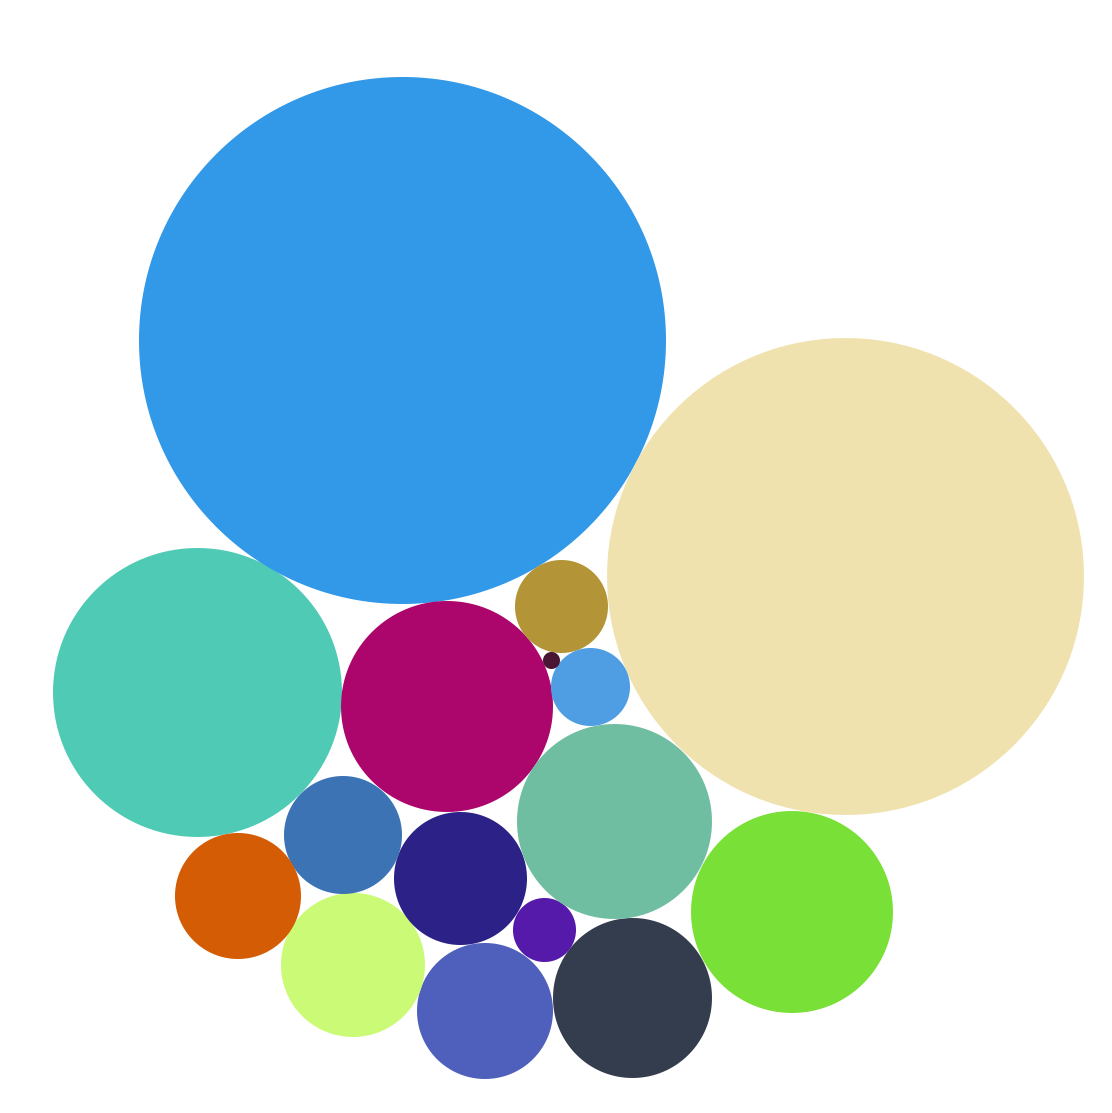
\includegraphics[width=180pt]{images/CP1.png}
\end{center}



\end{frame}




\begin{frame}
\frametitle{2. ~ Circle packings}


\begin{center}
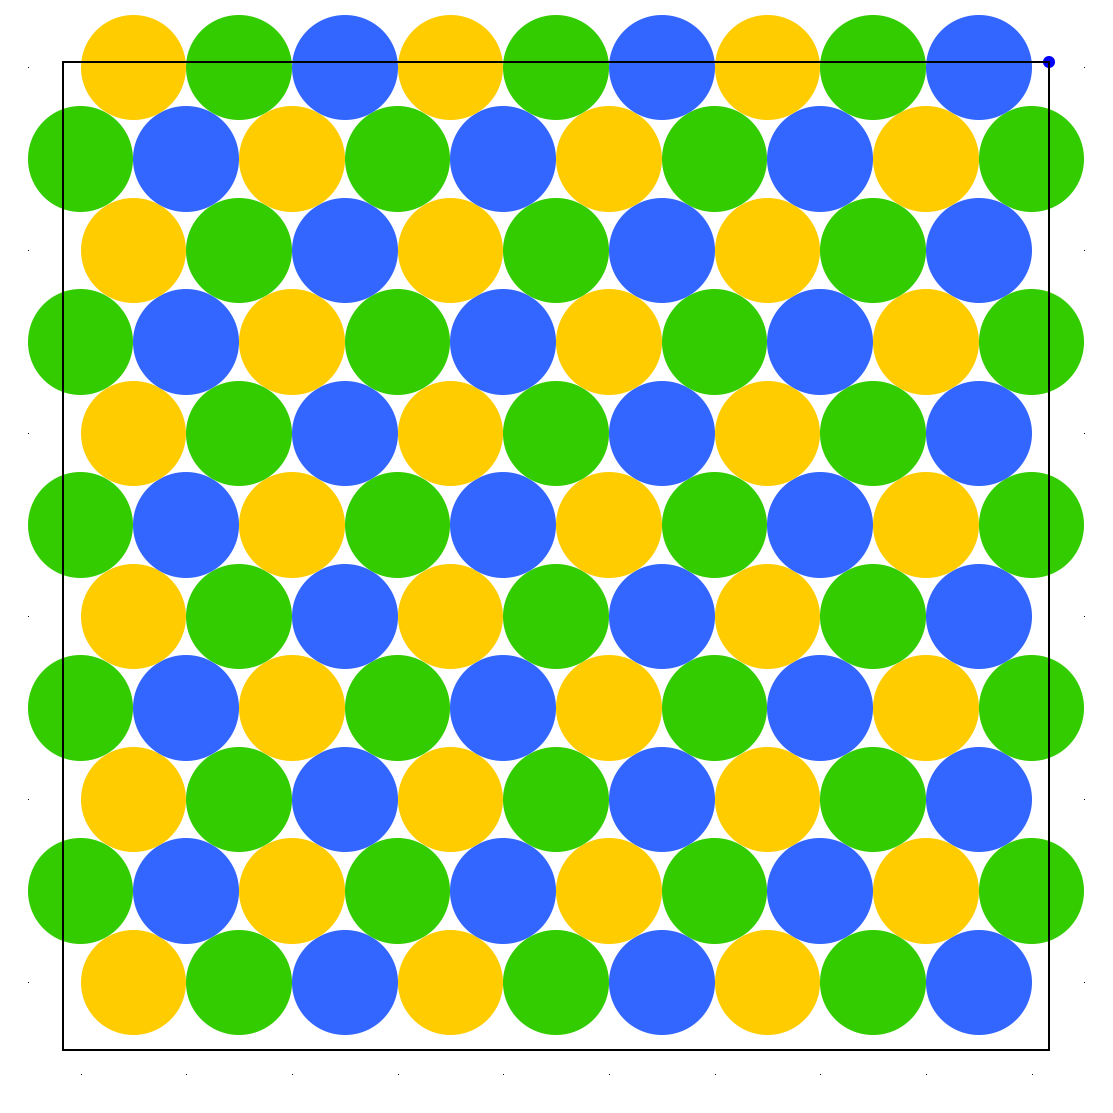
\includegraphics[width=130pt]{images/CP5.png} \hspace{30pt}
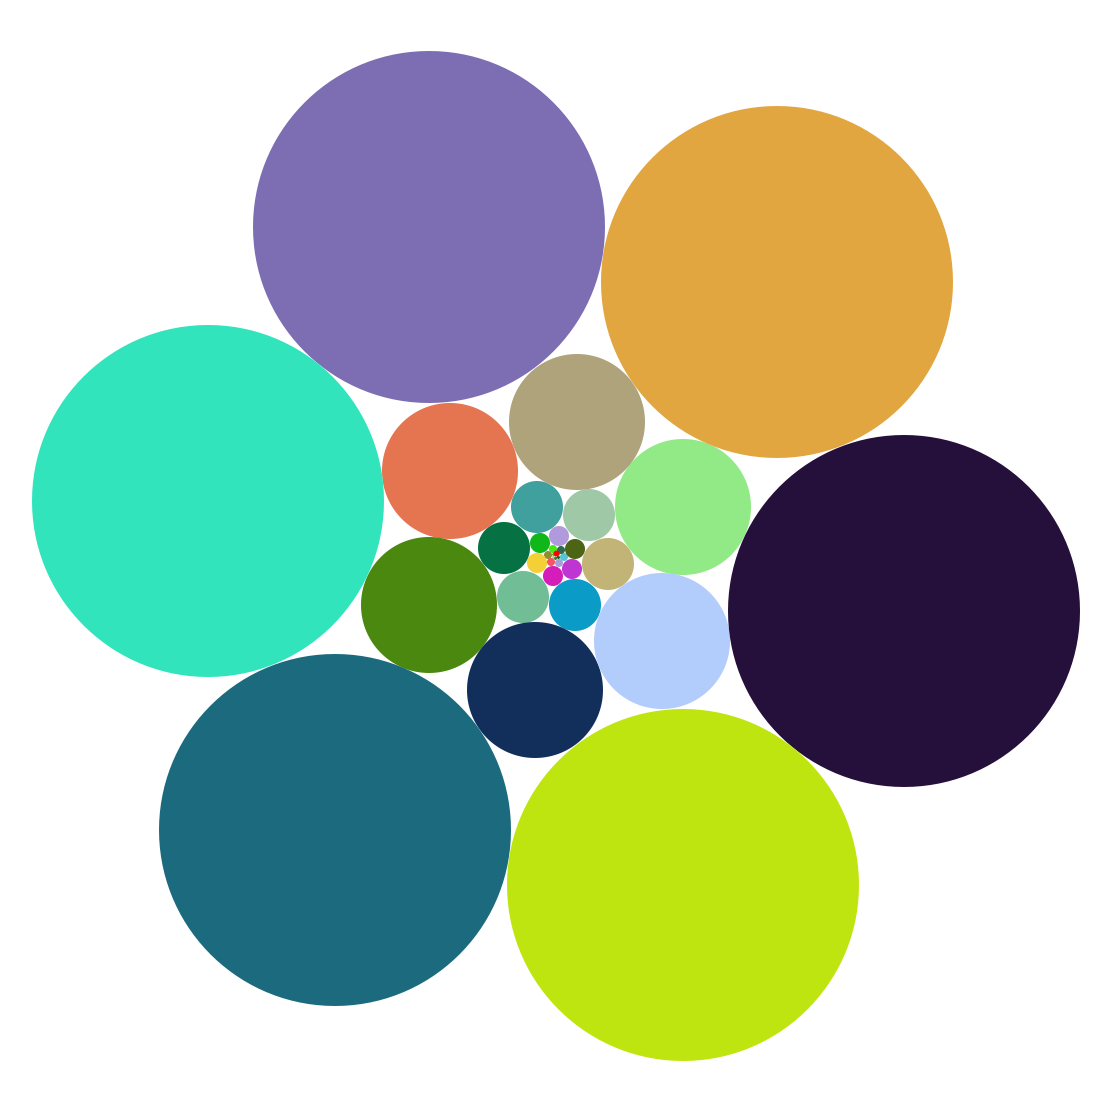
\includegraphics[width=130pt]{images/CP7.png}
\end{center}

\end{frame}






\begin{frame}
\frametitle{2. ~ Circle packings}



{\bfseries Apollonian gasket:}

\begin{center}
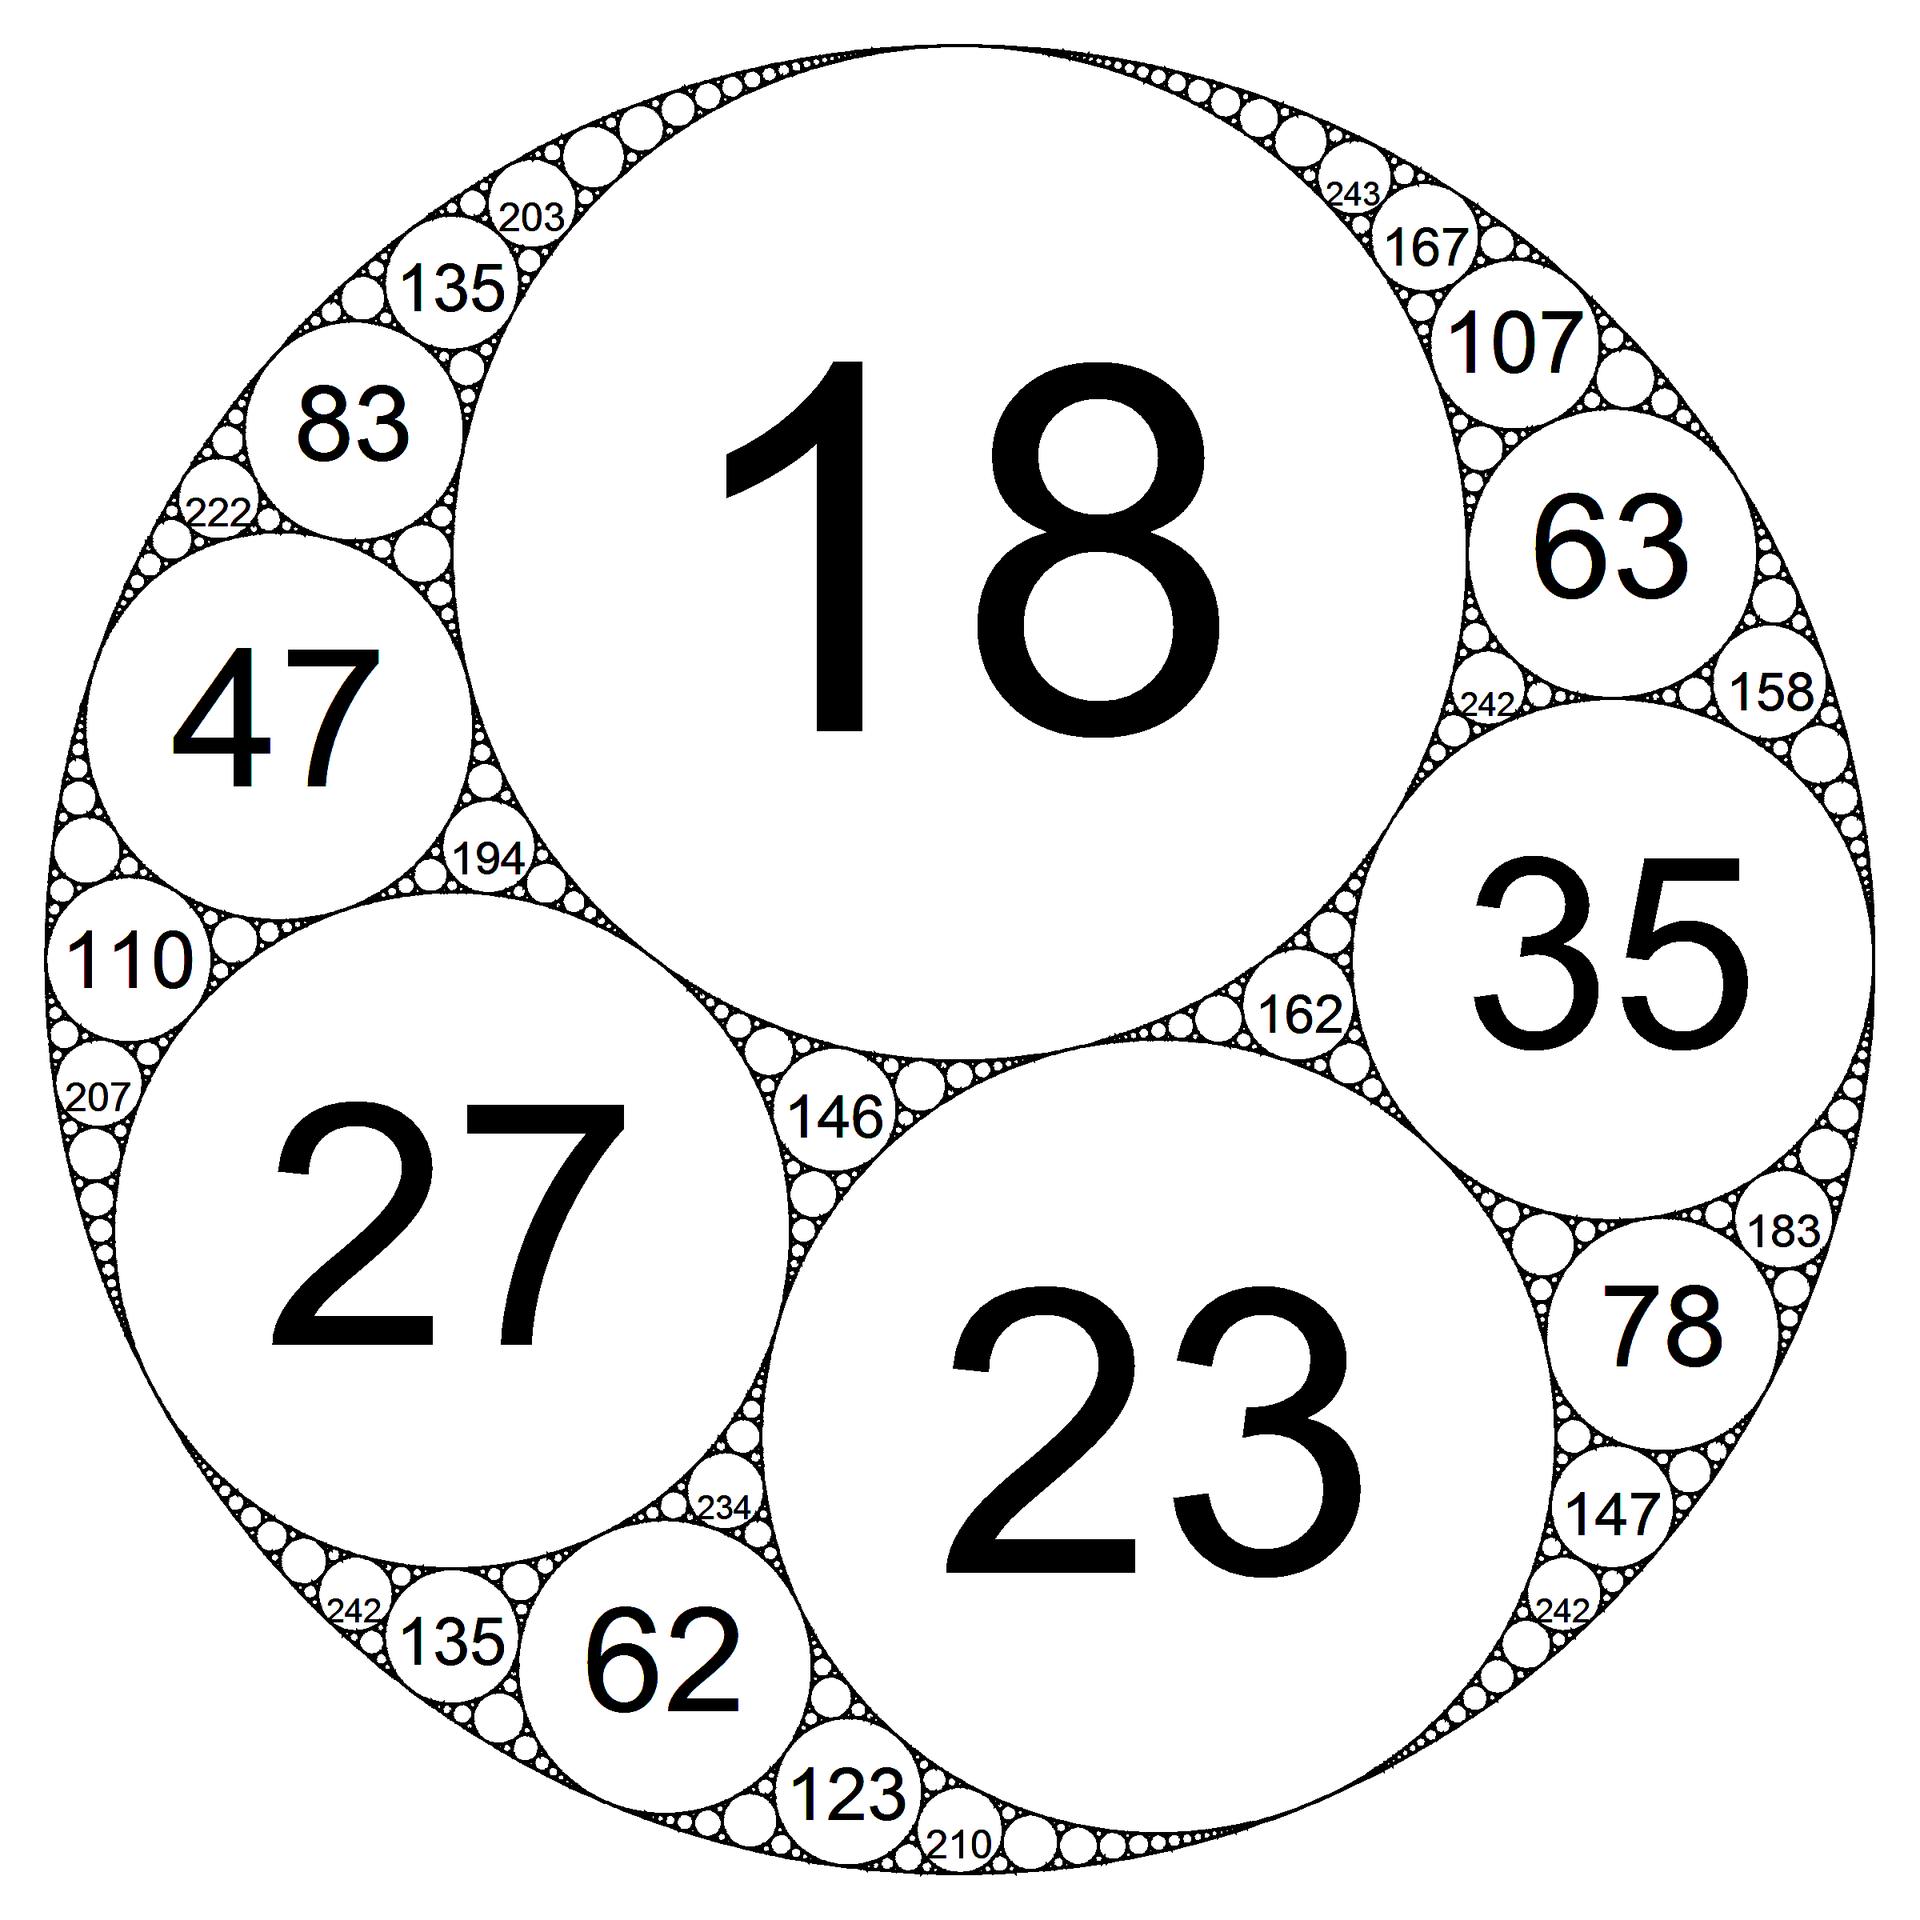
\includegraphics[width=170pt]{images/ApollonianGasket.png}
\end{center}

The curvatures (inverse radii) of four mutually tangent circles satisfy:
$(a + b + c + d)^2 = a^2 + b^2 + c^2 + d^2 $

\end{frame}



\begin{frame}
\frametitle{2. ~ Circle packings}



{\bfseries A circle packing defines a graph:} \pause
\begin{itemize}[$\bullet$]
 \item Vertices = circles
 \item Edges = tangency
\end{itemize}

\bigskip \pause

\begin{center}
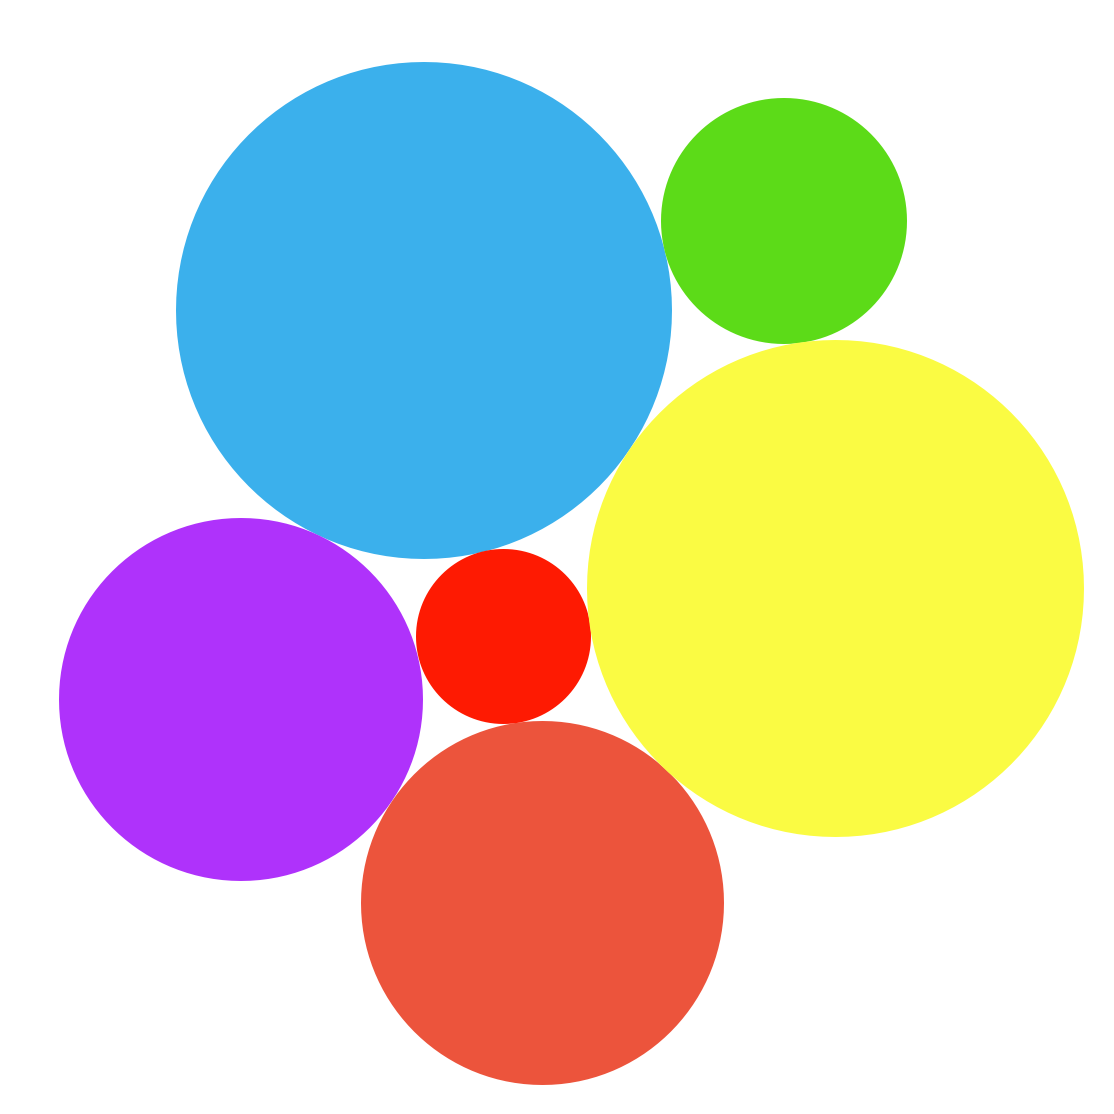
\includegraphics[width=120pt]{images/CP8b.png} \hspace{20pt} \pause
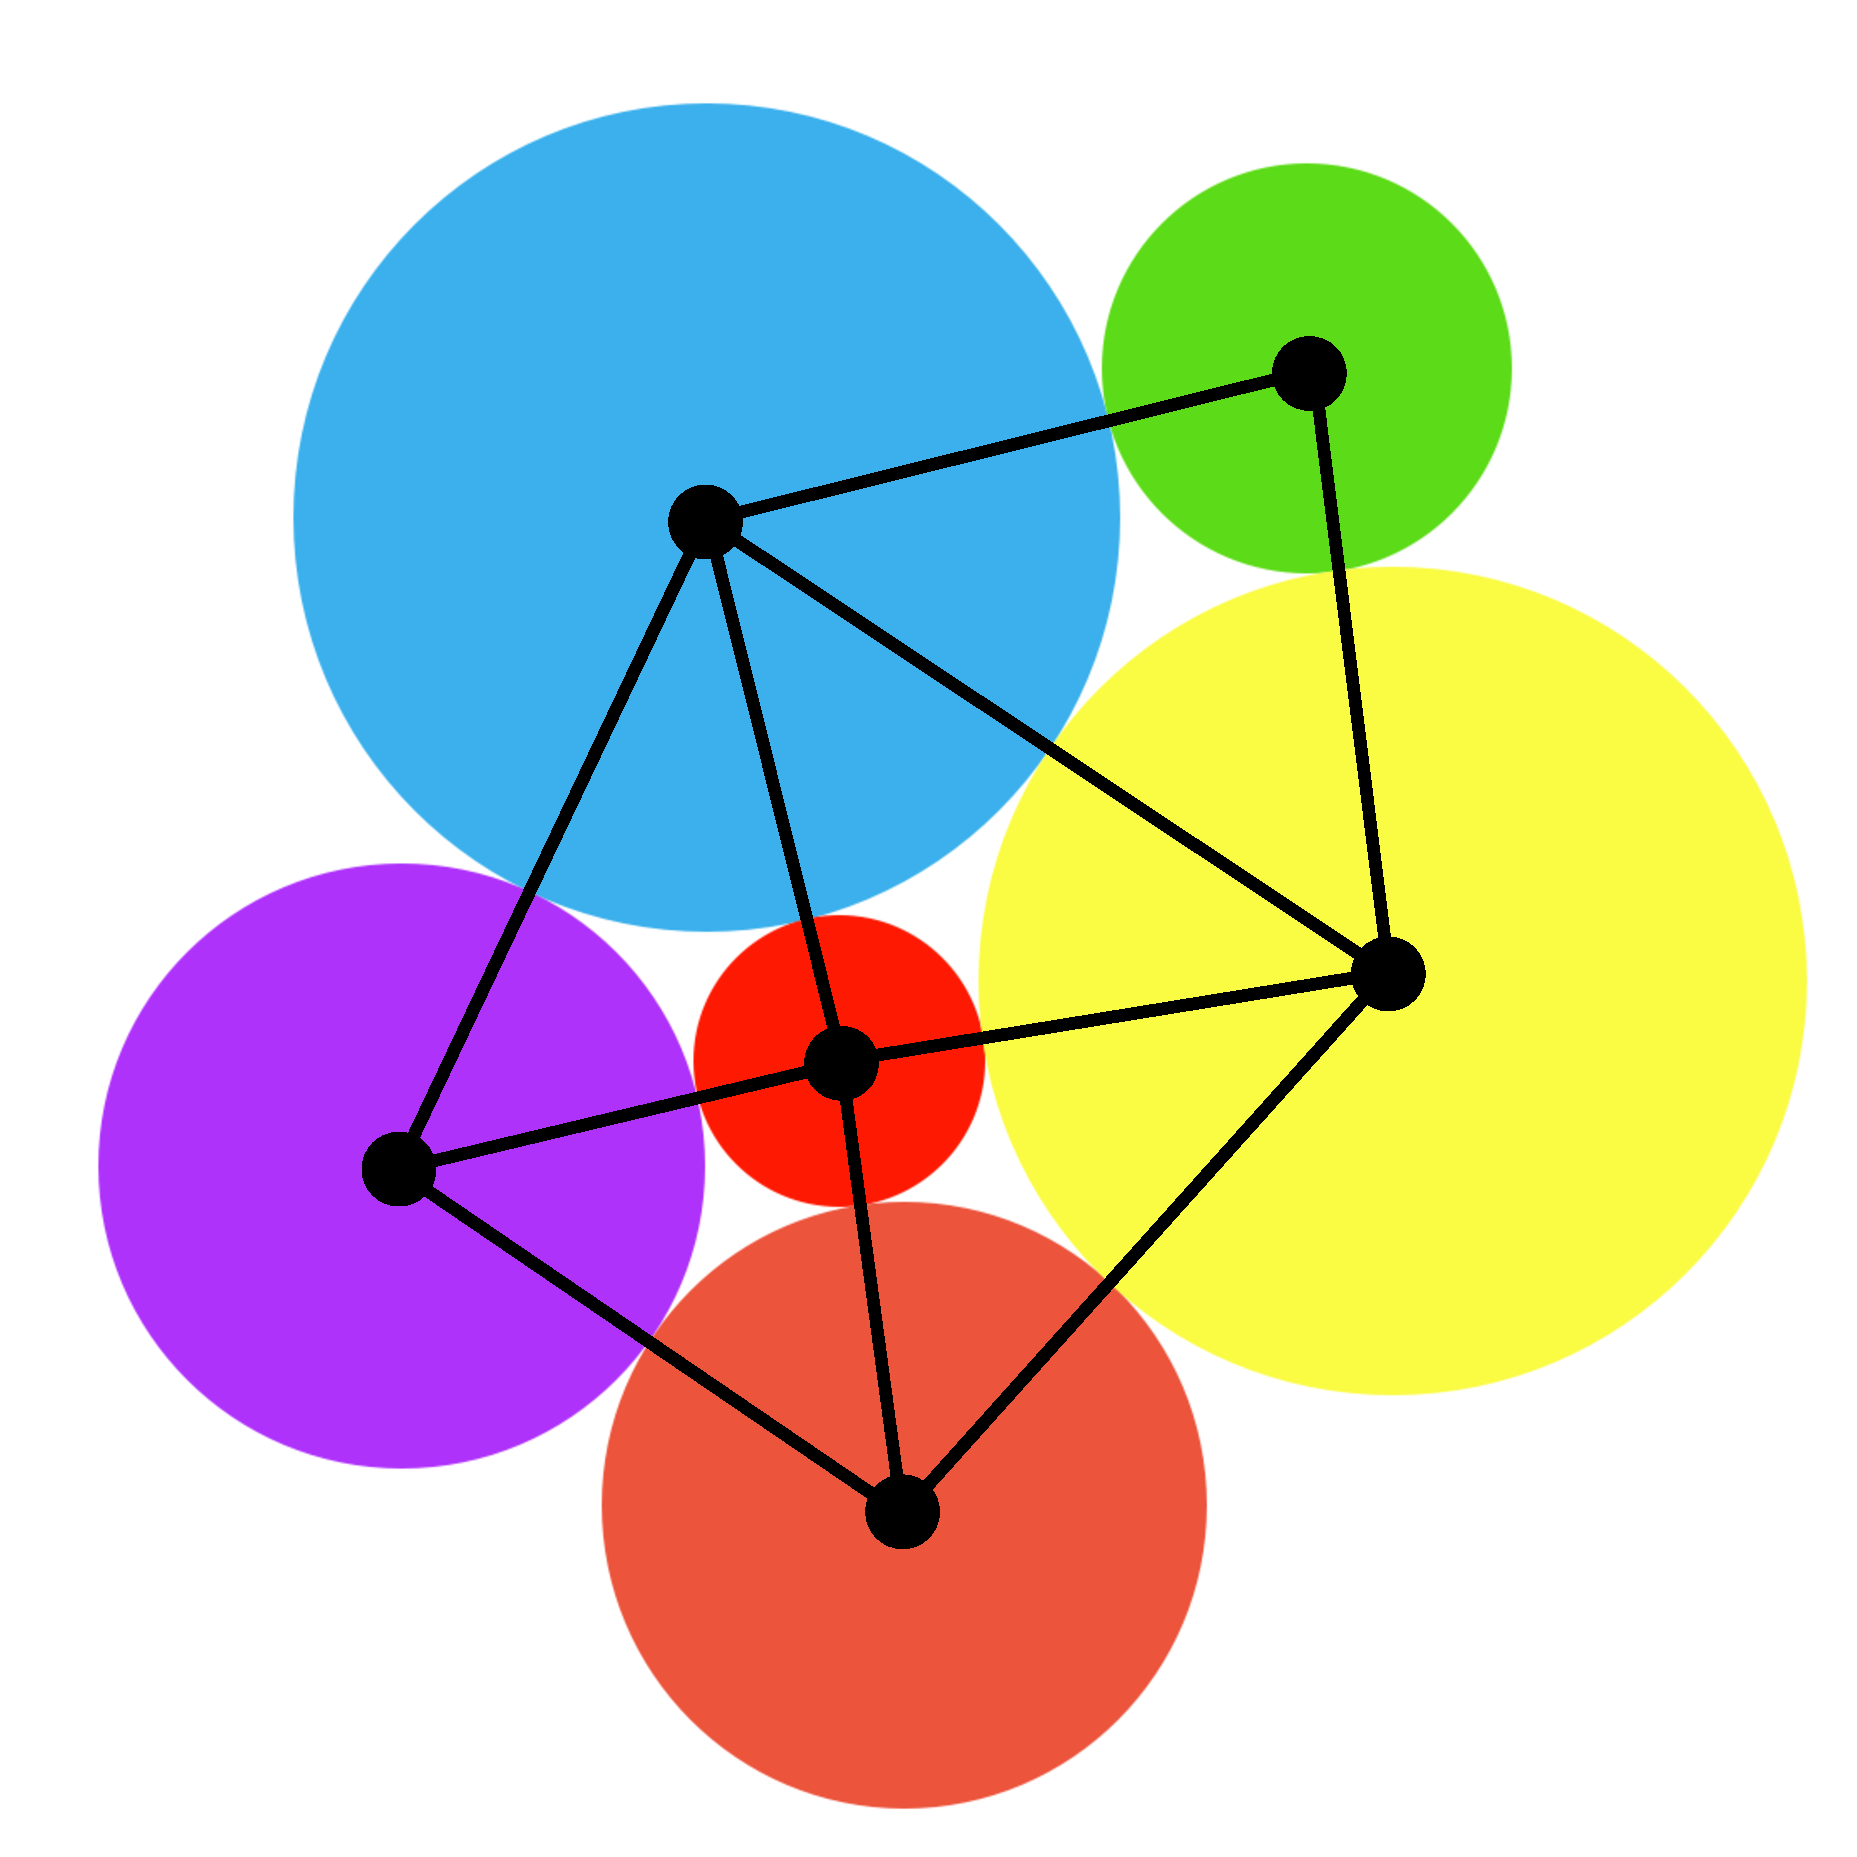
\includegraphics[width=120pt]{images/CP8c.pdf}
\end{center}

\end{frame}



\begin{frame}
\frametitle{2. ~ Circle packings}


\medskip 
Conversely, can one draw a circle packing realizing any planar graph?

\smallskip \pause
\begin{theorem}[Circle packing theorem]
\pause Yes.
\end{theorem}

\smallskip \pause
\emph{\small (Due to Koebe. Thurston: it is easily derived from Mostow rigidity for hyperbolic $3$-manifolds.)}



\medskip \pause
\begin{center}
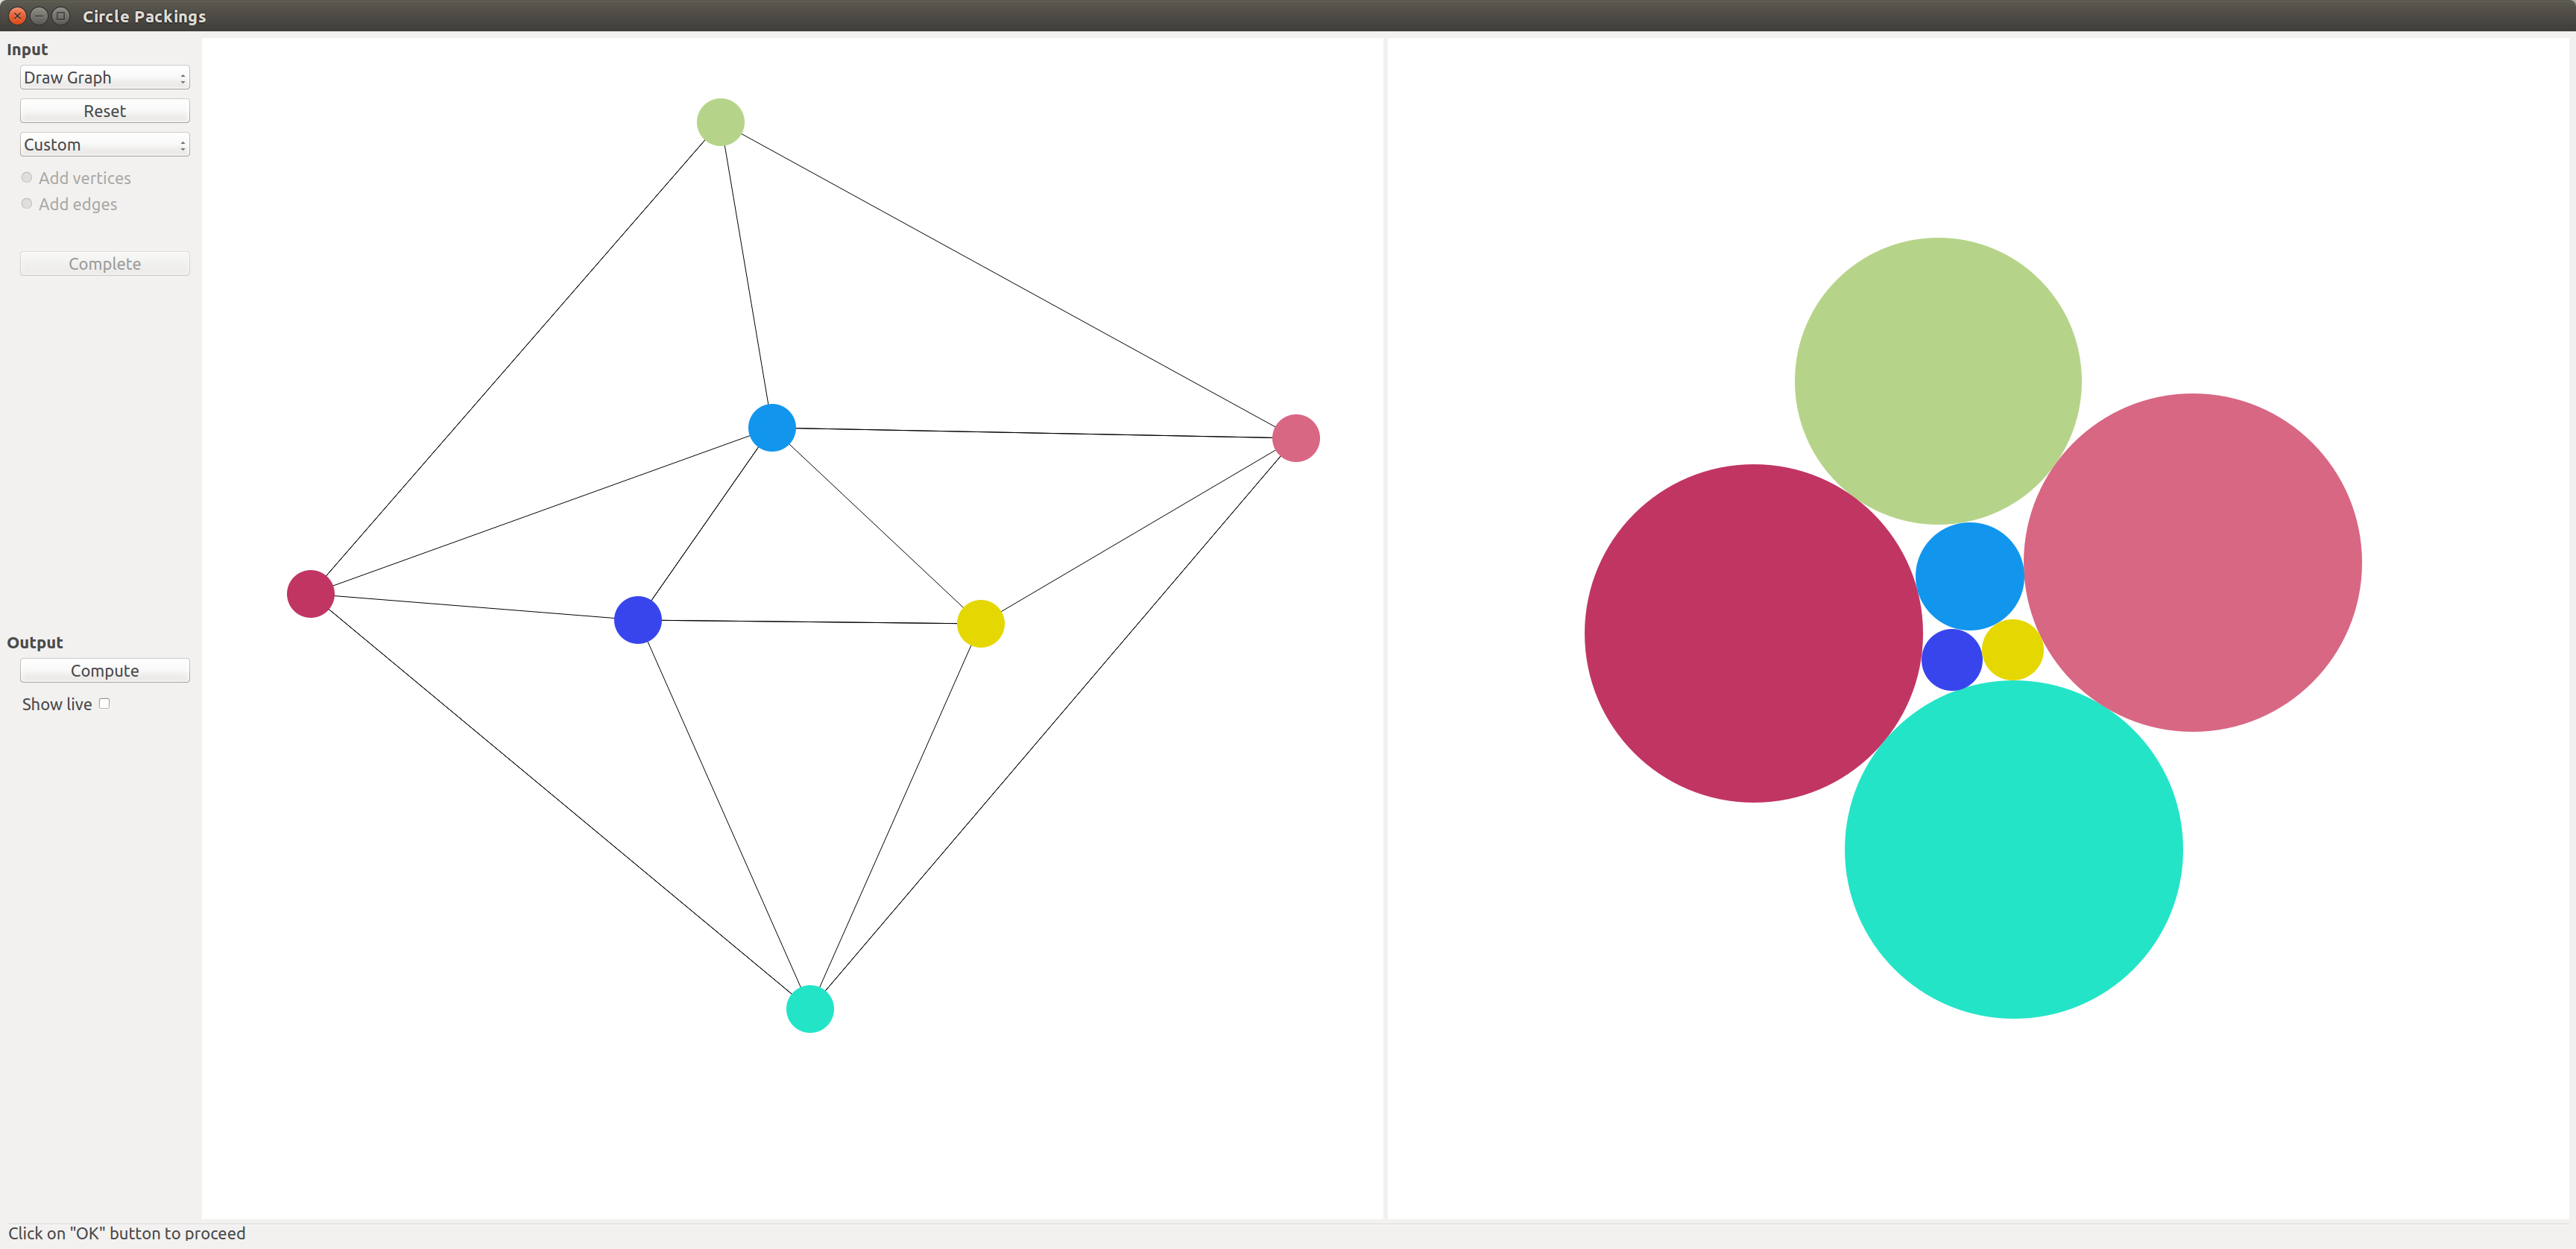
\includegraphics[width=\textwidth]{images/Screenshot1-c.png}
\end{center}

\end{frame}
